\documentclass[11pt,a4paper]{article}
\usepackage[backend=biber]{biblatex}
\usepackage{graphicx}
\usepackage{subcaption}
\usepackage{pgfplots}
\usepackage[top=1in, bottom=1.25in, left=0.5in, right=0.5in]{geometry}

\addbibresource{references.bib}
\pgfplotsset{compat=1.15}

\begin{document}

\title{Fault Detection}
\author{Danil Kuzin}
\date{January-March 2019}
\maketitle

\abstract
This report presents the results of the work done for geological faults detection with deep learning methods.



\section{Introduction}

The relevant literature includes: training CNNs on synthetic and real seismic data for faults detection~\cite{pochet2018seismic, araya2017automated, xiong2018seismic, chehrazi2013seismic, lu2018using}

The other literature on detection from satellite images includes: detecting roads on pixel level from lots of satellite images and then denoising to get connected nets \cite{mnih2010learning},

The potential extensions of this work can include synthetic data, that is described in~\cite{hale2014}.

\section{Data}

We use the satellite images from the Landsat-8 and elevation data from the Opentopography:  Shuttle Radar Topography Mission (SRTM GL1) Global 30m. The additional band is the slope estimated based on elevation.
The full list of features is:
\begin{itemize}
\item \textit{Optical R, G, B}
\item \textit{elevation}
\item \textit{slope}
\item \textit{ultrablue}
\item \textit{nir}
\item \textit{swir1}
\item \textit{swir2}
\item \textit{panchromatic}
\item \textit{erosion}
\item \textit{curvature}
\end{itemize}
The features are normalised separately for every region.

The faults and fault lookalikes were labelled on some of the regions.

The examples of labelled data and bands are shown in the \figurename~\ref{fig:features}
\begin{figure}[t]
    \centering
    \begin{subfigure}[b]{0.18\textwidth}
        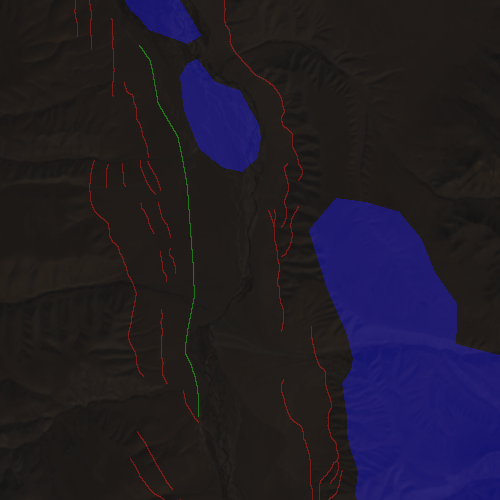
\includegraphics[width=\textwidth]{graphics/data/0/features_optical_rgb.png}
        \caption{Optical RGB}
        \label{fig:features_optical_rgb}
    \end{subfigure}
    ~
    \begin{subfigure}[b]{0.18\textwidth}
        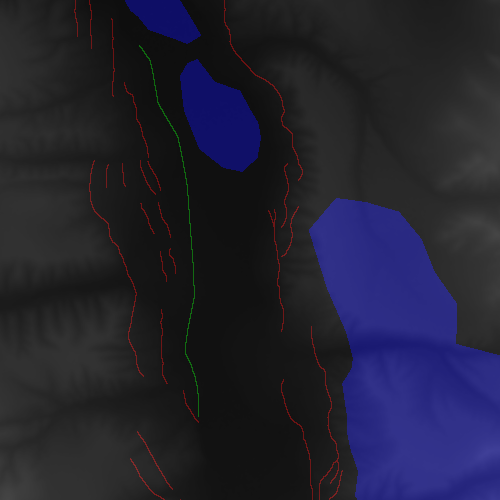
\includegraphics[width=\textwidth]{graphics/data/0/features_elevation.png}
        \caption{Elevation}
        \label{fig:features_elevation}
    \end{subfigure}
    ~
    \begin{subfigure}[b]{0.18\textwidth}
        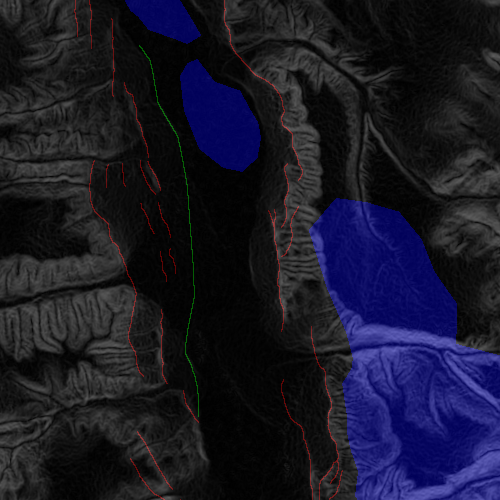
\includegraphics[width=\textwidth]{graphics/data/0/features_slope.png}
        \caption{Slope}
        \label{fig:features_slope}
    \end{subfigure}
    ~
    \begin{subfigure}[b]{0.18\textwidth}
        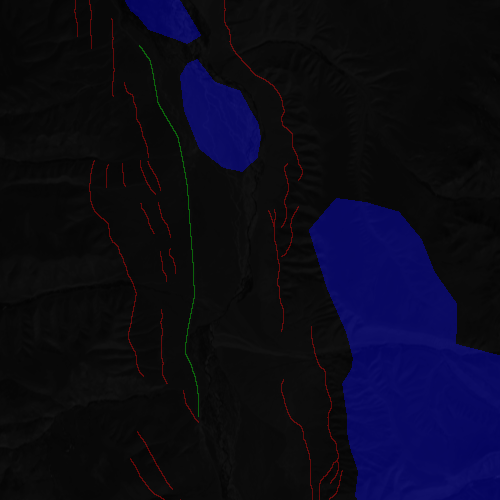
\includegraphics[width=\textwidth]{graphics/data/0/features_ultrablue.png}
        \caption{Ultrablue}
        \label{fig:features_ultrablue}
    \end{subfigure}
    ~
    \begin{subfigure}[b]{0.18\textwidth}
        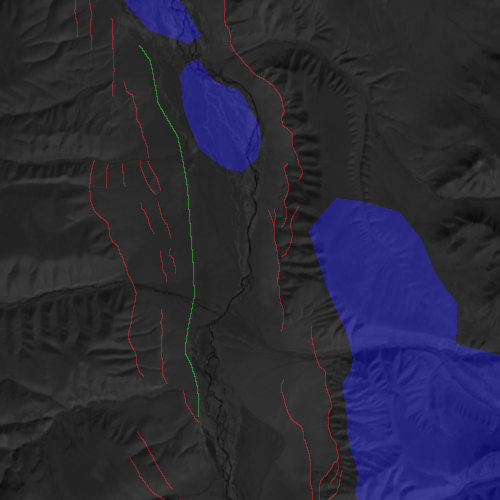
\includegraphics[width=\textwidth]{graphics/data/0/features_nir.png}
        \caption{Nir}
        \label{fig:features_nir}
    \end{subfigure}

    \begin{subfigure}[b]{0.18\textwidth}
        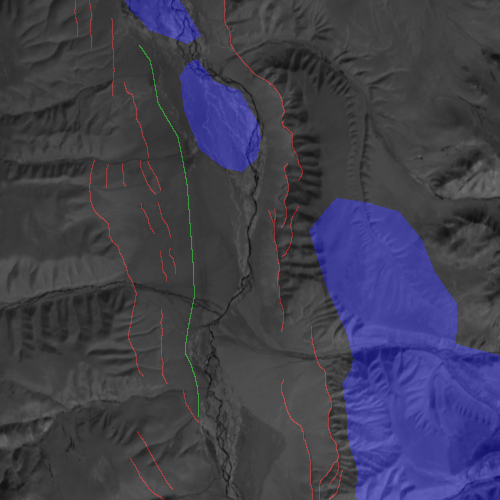
\includegraphics[width=\textwidth]{graphics/data/0/features_swir1.png}
        \caption{Swir1}
        \label{fig:features_swir1}
    \end{subfigure}
    ~
    \begin{subfigure}[b]{0.18\textwidth}
        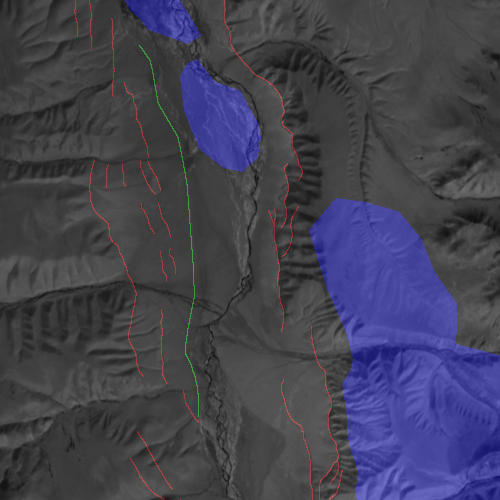
\includegraphics[width=\textwidth]{graphics/data/0/features_swir2.png}
        \caption{swir2}
        \label{fig:features_swir2}
    \end{subfigure}
    ~
    \begin{subfigure}[b]{0.18\textwidth}
        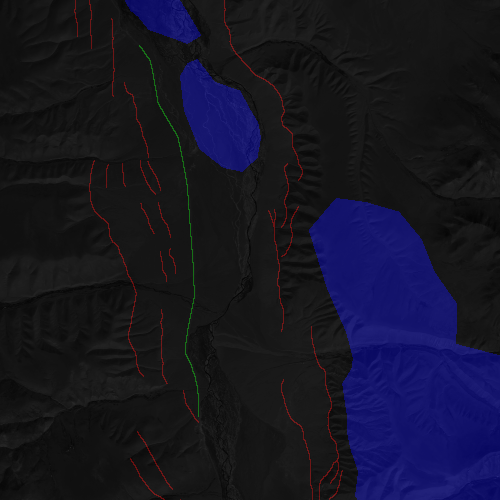
\includegraphics[width=\textwidth]{graphics/data/0/features_panchromatic.png}
        \caption{panchromatic}
        \label{fig:features_panchromatic}
    \end{subfigure}
    ~
    \begin{subfigure}[b]{0.18\textwidth}
        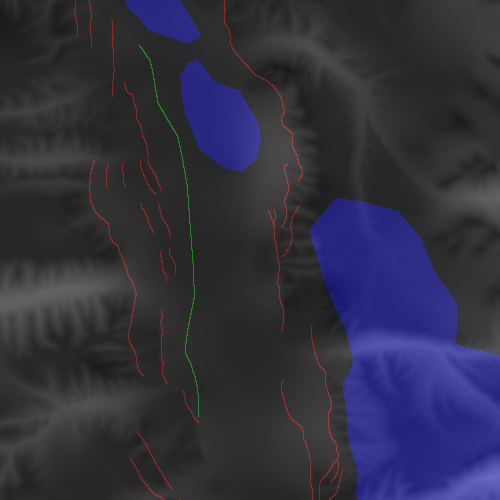
\includegraphics[width=\textwidth]{graphics/data/0/features_erosion.png}
        \caption{erosion}
        \label{fig:features_erosion}
    \end{subfigure}
    ~
    \begin{subfigure}[b]{0.18\textwidth}
        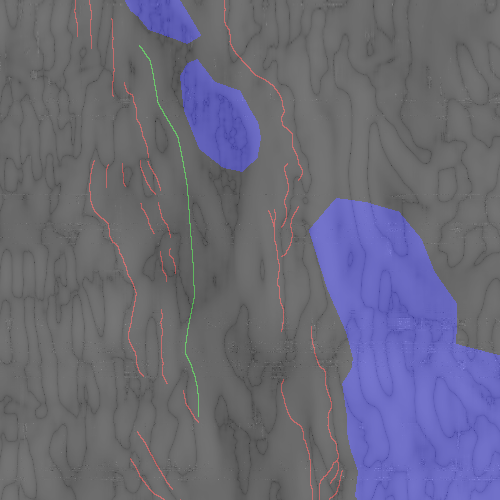
\includegraphics[width=\textwidth]{graphics/data/0/features_curve.png}
        \caption{curve}
        \label{fig:features_curve}
    \end{subfigure}
    \caption{Labelled features for a subset of data}\label{fig:features}
\end{figure}

\section{Neural network}
We base the architecture on the LeNet-5 net~\cite{lecun1998gradient}:
\begin{enumerate}
\item \textit{Input Layer} of shape $patch_width \times patch_height \times num-of-features$
\item \textit{2D convolution} with $32$ filters of $5 \times 5$ kernel size
\item \textit{Relu} activation
\item \textit{MaxPooling2D} with $2 \times 2$ pool size
\item \textit{2D convolution} with 64 filters of $5 \times 5$ kernel size
\item \textit{Relu} activation
\item \textit{MaxPooling2D} with $2 \times 2$ pool size
\item \textit{Flatten} layer
\item \textit{Dense} with $1024$ units
\item \textit{relu} activation
\item \textit{Dropout} with $0.5$ rate
\item \textit{Dense} layer with $2$ units corresponding to output classes
\item \textit{Softmax} activation
\end{enumerate}
Categorical crossentropy is used for loss estimation.

Experiments with higher (up to 5 convolutional) number of layers demonstrated that the current amount of training data
is not enough to utilise the advantages of more complex architectures.

\section{Experiments}
For training we use the data, sampled randomly from training images. Faults and fault lookalikes are marked with lines,
we sample random points from these lines and create patches of shape $(150 x 150)$ with centers at these points.
Non-fault areas are marked with polygons, we sample patches that fully lie within the marked polygon.

During training, we perform 10 epochs of 50 iterations each. At every iteration a minibatch of 10 patches is sampled
from the regions, randomly rotated and flipped.

\subsection{Train on Tibet data}
\begin{figure}
\begin{tikzpicture}
\begin{axis}[axis lines=left, xlabel=epoch, legend pos=outer north east]
\addplot[solid, color=orange, mark=*, mark options={solid}] table[x=epoch, y=val_acc, col sep=comma] {graphics/training/train_on_01_features_01234_no_additional/log.csv};
\addlegendentry{val acc}
\addplot[dashed, color=orange, mark=*, mark options={solid}] table[x=epoch, y=acc, col sep=comma] {graphics/training/train_on_01_features_01234_no_additional/log.csv};
\addlegendentry{acc}
\addplot[solid, color=cyan, mark=*, mark options={solid}] table [x=epoch, y=val_loss, col sep=comma] {graphics/training/train_on_01_features_01234_no_additional/log.csv};
\addlegendentry{val loss}
\addplot[dashed, color=cyan, mark=*, mark options={solid}] table [x=epoch, y=loss, col sep=comma] {graphics/training/train_on_01_features_01234_no_additional/log.csv};
\addlegendentry{loss}
\end{axis}
\end{tikzpicture}
\label{train_on_016_features_01234_no_additional}
\caption{training on Tibet data and validating on a US region}
\end{figure}

\begin{figure}[t]
    \centering
    \begin{subfigure}[b]{0.12\textwidth}
        \includegraphics[width=\textwidth]{graphics/training/train_on_01_features_01234_no_additional/heatmaps_faults_0.png}
        \caption{Lopukangri}
        \label{fig:heatmaps_2_Lopukangri}
    \end{subfigure}
    ~
    \begin{subfigure}[b]{0.12\textwidth}
        \includegraphics[width=\textwidth]{graphics/training/train_on_01_features_01234_no_additional/heatmaps_faults_1.png}
        \caption{Muga Puruo}
        \label{fig:heatmaps_2_Muga_Puruo}
    \end{subfigure}
    ~
    \begin{subfigure}[b]{0.12\textwidth}
        \includegraphics[width=\textwidth]{graphics/training/train_on_01_features_01234_no_additional/heatmaps_faults_2.png}
        \caption{Muggarboibo}
        \label{fig:heatmaps_2_Muggarboibo}
    \end{subfigure}
    ~
    \begin{subfigure}[b]{0.12\textwidth}
        \includegraphics[width=\textwidth]{graphics/training/train_on_01_features_01234_no_additional/heatmaps_faults_3.png}
        \caption{Austin-Tonopah}
        \label{fig:heatmaps_2_Austin-Tonopah}
    \end{subfigure}
    ~
    \begin{subfigure}[b]{0.12\textwidth}
        \includegraphics[width=\textwidth]{graphics/training/train_on_01_features_01234_no_additional/heatmaps_faults_4.png}
        \caption{Las Vegas Nevada}
        \label{fig:heatmaps_2_Las_Vegas_Nevada}
    \end{subfigure}
    ~
    \begin{subfigure}[b]{0.12\textwidth}
        \includegraphics[width=\textwidth]{graphics/training/train_on_01_features_01234_no_additional/heatmaps_faults_5.png}
        \caption{Izmir Turkey}
        \label{fig:heatmaps_2_Izmir_Turkey}
    \end{subfigure}
    ~
    \begin{subfigure}[b]{0.12\textwidth}
        \includegraphics[width=\textwidth]{graphics/training/train_on_01_features_01234_no_additional/heatmaps_faults_6.png}
        \caption{Nevada}
        \label{fig:heatmaps_2_Nevada}
    \end{subfigure}

    \caption{Predictions, heatmaps}\label{fig:train_on_01_features_01234_no_additional_im}
\end{figure}

\subsection{Train on US data}
\begin{figure}
\begin{tikzpicture}
\begin{axis}[axis lines=left, xlabel=epoch, legend pos=outer north east]
\addplot[solid, color=orange, mark=*, mark options={solid}] table[x=epoch, y=val_acc, col sep=comma] {graphics/training/train_on_6_features_01234_no_additional/log.csv};
\addlegendentry{val acc}
\addplot[dashed, color=orange, mark=*, mark options={solid}] table[x=epoch, y=acc, col sep=comma] {graphics/training/train_on_6_features_01234_no_additional/log.csv};
\addlegendentry{acc}
\addplot[solid, color=cyan, mark=*, mark options={solid}] table [x=epoch, y=val_loss, col sep=comma] {graphics/training/train_on_6_features_01234_no_additional/log.csv};
\addlegendentry{val loss}
\addplot[dashed, color=cyan, mark=*, mark options={solid}] table [x=epoch, y=loss, col sep=comma] {graphics/training/train_on_6_features_01234_no_additional/log.csv};
\addlegendentry{loss}
\end{axis}
\end{tikzpicture}
\label{train_on_6_features_01234_no_additional}
\caption{training on US data and validating on a different US region}
\end{figure}

\begin{figure}[t]
    \centering
    \begin{subfigure}[b]{0.12\textwidth}
        \includegraphics[width=\textwidth]{graphics/training/train_on_6_features_01234_no_additional/heatmaps_faults_0.png}
        \caption{Lopukangri}
        \label{fig:heatmaps_3_Lopukangri}
    \end{subfigure}
    ~
    \begin{subfigure}[b]{0.12\textwidth}
        \includegraphics[width=\textwidth]{graphics/training/train_on_6_features_01234_no_additional/heatmaps_faults_1.png}
        \caption{Muga Puruo}
        \label{fig:heatmaps_3_Muga_Puruo}
    \end{subfigure}
    ~
    \begin{subfigure}[b]{0.12\textwidth}
        \includegraphics[width=\textwidth]{graphics/training/train_on_6_features_01234_no_additional/heatmaps_faults_2.png}
        \caption{Muggarboibo}
        \label{fig:heatmaps_3_Muggarboibo}
    \end{subfigure}
    ~
    \begin{subfigure}[b]{0.12\textwidth}
        \includegraphics[width=\textwidth]{graphics/training/train_on_6_features_01234_no_additional/heatmaps_faults_3.png}
        \caption{Austin-Tonopah}
        \label{fig:heatmaps_3_Austin-Tonopah}
    \end{subfigure}
    ~
    \begin{subfigure}[b]{0.12\textwidth}
        \includegraphics[width=\textwidth]{graphics/training/train_on_6_features_01234_no_additional/heatmaps_faults_4.png}
        \caption{Las Vegas Nevada}
        \label{fig:heatmaps_3_Las_Vegas_Nevada}
    \end{subfigure}
    ~
    \begin{subfigure}[b]{0.12\textwidth}
        \includegraphics[width=\textwidth]{graphics/training/train_on_6_features_01234_no_additional/heatmaps_faults_5.png}
        \caption{Izmir Turkey}
        \label{fig:heatmaps_3_Izmir_Turkey}
    \end{subfigure}


    \caption{Predictions, heatmaps}\label{fig:train_on_6_features_01234_no_additional_im}
\end{figure}


\subsection{Training on Tibet and US data jointly}
\begin{figure}
\begin{tikzpicture}
\begin{axis}[axis lines=left, xlabel=epoch, legend pos=outer north east]
\addplot[solid, color=orange, mark=*, mark options={solid}] table[x=epoch, y=val_acc, col sep=comma] {graphics/training/train_on_016_features_01234_no_additional/log.csv};
\addlegendentry{val acc}
\addplot[dashed, color=orange, mark=*, mark options={solid}] table[x=epoch, y=acc, col sep=comma] {graphics/training/train_on_016_features_01234_no_additional/log.csv};
\addlegendentry{acc}
\addplot[solid, color=cyan, mark=*, mark options={solid}] table [x=epoch, y=val_loss, col sep=comma] {graphics/training/train_on_016_features_01234_no_additional/log.csv};
\addlegendentry{val loss}
\addplot[dashed, color=cyan, mark=*, mark options={solid}] table [x=epoch, y=loss, col sep=comma] {graphics/training/train_on_016_features_01234_no_additional/log.csv};
\addlegendentry{loss}
\end{axis}
\end{tikzpicture}
\label{train_on_016_features_01234_no_additional}
\caption{training on tibet and US data and validating on a different US region}
\end{figure}

\figurename~\ref{train_on_016_features_01234_no_additional} contains the quality metrics during training,
\figurename~\ref{fig:train_on_016_features_01234_no_additional_im} contains the example predictions for different regions

\begin{figure}[t]
    \centering
    \begin{subfigure}[b]{0.12\textwidth}
        \includegraphics[width=\textwidth]{graphics/training/train_on_016_features_01234_no_additional/heatmaps_faults_0.png}
        \caption{Lopukangri}
        \label{fig:heatmaps_1_Lopukangri}
    \end{subfigure}
    ~
    \begin{subfigure}[b]{0.12\textwidth}
        \includegraphics[width=\textwidth]{graphics/training/train_on_016_features_01234_no_additional/heatmaps_faults_1.png}
        \caption{Muga Puruo}
        \label{fig:heatmaps_1_Muga_Puruo}
    \end{subfigure}
    ~
    \begin{subfigure}[b]{0.12\textwidth}
        \includegraphics[width=\textwidth]{graphics/training/train_on_016_features_01234_no_additional/heatmaps_faults_2.png}
        \caption{Muggarboibo}
        \label{fig:heatmaps_1_Muggarboibo}
    \end{subfigure}
    ~
    \begin{subfigure}[b]{0.12\textwidth}
        \includegraphics[width=\textwidth]{graphics/training/train_on_016_features_01234_no_additional/heatmaps_faults_3.png}
        \caption{Austin-Tonopah}
        \label{fig:heatmaps_1_Austin-Tonopah}
    \end{subfigure}
    ~
    \begin{subfigure}[b]{0.12\textwidth}
        \includegraphics[width=\textwidth]{graphics/training/train_on_016_features_01234_no_additional/heatmaps_faults_4.png}
        \caption{Las Vegas Nevada}
        \label{fig:heatmaps_1_Las_Vegas_Nevada}
    \end{subfigure}
    ~
    \begin{subfigure}[b]{0.12\textwidth}
        \includegraphics[width=\textwidth]{graphics/training/train_on_016_features_01234_no_additional/heatmaps_faults_5.png}
        \caption{Izmir Turkey}
        \label{fig:heatmaps_1_Izmir_Turkey}
    \end{subfigure}
    ~
    \begin{subfigure}[b]{0.12\textwidth}
        \includegraphics[width=\textwidth]{graphics/training/train_on_016_features_01234_no_additional/heatmaps_faults_6.png}
        \caption{Nevada}
        \label{fig:heatmaps_1_Nevada}
    \end{subfigure}

    \caption{Predictions, heatmaps}\label{fig:train_on_016_features_01234_no_additional_im}
\end{figure}

\section{NN visualisations}

\section{Future work}
\begin{itemize}
\item Increasing the amount of data that we have may allow to increase the architecture of the network, receptive
fields of the convolutions on later layers may provide more meaningful visualisations.
\item preprocessing can include further random transformations: well-established optical transforms, such as changing
brightness and contrast, cropping. For other bands the methods are not explored in the literature.
\end{itemize}
\printbibliography

\end{document}